\documentclass[titlepage = firstcover]{scrartcl}
\usepackage[aux]{rerunfilecheck}
\usepackage{fontspec}
\usepackage[main=ngerman, english, french]{babel}

% mehr Pakete hier
\usepackage{expl3}
\usepackage{xparse}
\usepackage{pdfpages}

%Mathematik------------------------------------------------------
\usepackage{amsmath}   % unverzichtbare Mathe-Befehle
\usepackage{amssymb}   % viele Mathe-Symbole
\usepackage{mathtools} % Erweiterungen für amsmath
\usepackage[
  math-style=ISO,    % \
  bold-style=ISO,    % |
  sans-style=italic, % | ISO-Standard folgen
  nabla=upright,     % |
  partial=upright,   % /
]{unicode-math}% "Does exactly what it says on the tin."
\usepackage[section, below]{placeins}
\usepackage{upgreek}

% Laden von OTF-Mathefonts
% Ermöglich Unicode Eingabe von Zeichen: α statt \alpha

\setmathfont{Latin Modern Math}
%\setmathfont{Tex Gyre Pagella Math} % alternativ zu Latin Modern Math
\setmathfont{XITS Math}[range={scr, bfscr}]
\setmathfont{XITS Math}[range={cal, bfcal}, StylisticSet=1]


\AtBeginDocument{ % wird bei \begin{document}
  % werden sonst wieder von unicode-math überschrieben
  \RenewDocumentCommand \Re {} {\operatorname{Re}}
  \RenewDocumentCommand \Im {} {\operatorname{Im}}
}
\usepackage{mleftright}
\setlength{\delimitershortfall}{-1sp}

%Sprache----------------------------------------------------------
\usepackage{microtype}
\usepackage{xfrac}
\usepackage[autostyle]{csquotes}    % babel
\usepackage[german, unicode, pdfusetitle]{hyperref}
\usepackage{bookmark}
\usepackage[shortcuts]{extdash}
%Römische Zahlen großgeschrieben
\newcommand{\RN}[1]{\uppercase\expandafter{\romannumeral#1}}
%Einstellungen hier, z.B. Fonts
\usepackage{booktabs} % Tabellen
\usepackage{a4}
\usepackage{float}

\setlength{\parindent}{0pt}


\title{Geiger-Müller-Zählrohr}
\author{David Gutnikov \\
        \href{mailto:david.gutnikov@tu-dortmund.de}{david.gutnikov@tu-dortmund.de}}
\date{Abgabe am 25.05.2020}


\begin{document}

    \maketitle
    \newpage
    \tableofcontents
    \newpage

    \section{Zielsetzung}
      Es werden bei diesem Versuch die Charakteristik und die Totzeit eines Geiger-Müller-Zählrohrs bestimmt. Außerdem wird in Abhängigkeit von der Zählrohrspannung bestimmt wie viel Ladung pro einfallendem Teilchen freigesetzt wird.

    \section{Theorie}
      \subsection{Funktionsweise und Aufbau des Zählrohrs}
        Das Geiger-Müller-Zählrohr wird verwendet um die Intensität von ionisierender Strahlung zu messen. Unter diesem Begriff wird $\alpha$, $\beta$ und $\gamma$-Strahlung verstanden. Dabei haben $\alpha$-Teilchen das größte und $\gamma$-Quanten des kleinste spezifische Ionisationsvermögen. Je höher das spez. Ionisationsvermögen, desto mehr Ion-Elektron-Paare werden bei Durchgang durch ein Gas durch Stoßionisation pro zurückgelegte Strecke ionisiert (dazu später mehr). Bei Absorption der Strahlung durch das Gas werden elektrische Impulse erzeugt, welche dann gemessen werden.
        \subsubsection{Aufbau}
          \begin{figure}[h]
            \centering
            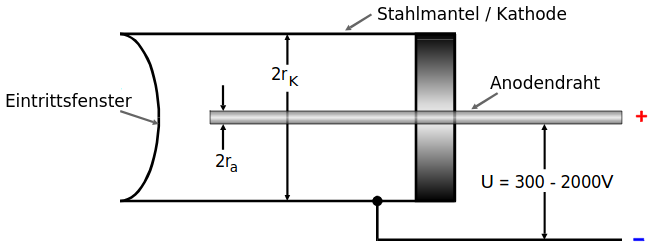
\includegraphics[width = 0.8\linewidth]{geiger_mueller_aufbau.png}
            \caption{Schematische Darstellung eines Geiger-Müller-Zählrohrs.}
            \label{fig:geiger-mueller-zaehlrohr}
          \end{figure}
          \FloatBarrier
              
          Innerhalb des Stahlmantels wird ein radialsymmetrisches elektrisches Feld aufgebaut, für das im Abstand $r$ vom Anodendraht gilt:
          \begin{equation}
              E(r) = \frac{U}{r \ln{\bigl(\sfrac{r_k}{r_a}}\bigr)}
              \label{eqn:feldstaerke}
          \end{equation}
          mit der angelegten Spannung $U$, dem Radius des Stahlzylinders $r_k$ und dem Radius des Anodendrahtes $r_a$.

        \subsubsection{Abhängigkeit der Ladungsimpulse von der Spannung}
          Kommt die Strahlung in das Zählrohr, trifft sie auf die Edelgasatome im Zylinder und ionisiert diese, sodass ein Elektron und ein positives Ion enstehen. Da die zur Erzeugung eines Ion-Elektron-Paares im Durchschnitt benötigte Energie 26 eV beträgt im Gegensatz zur Teilchenenergie in der Größenordnung von 100 keV sehr klein ist, ist die Anzahl der primär erzeugten Paare proportional zur Energie des einfallenden Teilchens. Die daraus weitergehenden Ionisierungsprozesse sind dahingegen stark von der Spannung abhängig. Deshalb kommt es in \autoref{fig:anzahl_spannung} zur Unterteilung in verschiedene Bereiche.
          \begin{figure}[h]
            \centering
            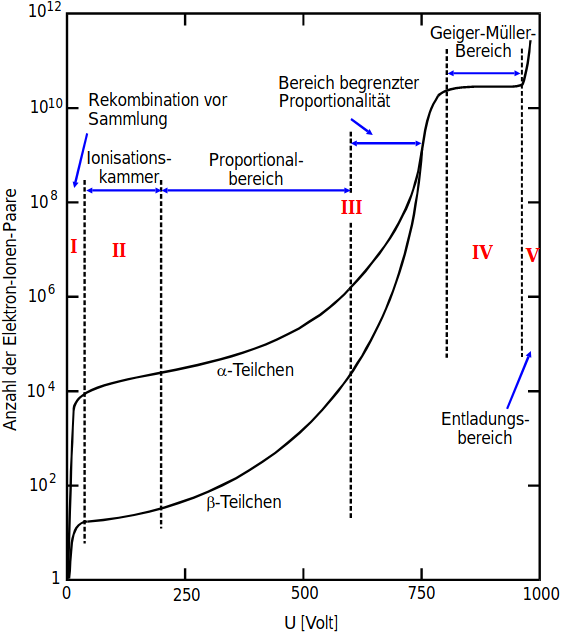
\includegraphics[width = 0.7\linewidth]{anzahl_spannung.png}
            \caption{Die Anzahl der erzeugten Ion-Elektron-Paare gegen die angelegte Spannung aufgetragen.}
            \label{fig:anzahl_spannung}
          \end{figure}
          \FloatBarrier

          \paragraph{Bereich \RN{1}:}
            Nur ein kleiner Teil der erzeugten Paare kommt am Anodendraht an, da sich der Rest wieder zu neutralen Atomen zusammenfügen. (Rekombination)

          \paragraph{Bereich \RN{2}:}
            Die Rekombinationswahrscheinlichkeit sinkt, weswegen jetzt fast alle erzeugten Elektronen am Draht ankommen. Der Ionisationsstrom ist proportional zur Energie und Intesität der einfallenden Strahlung. Doch da die Ladungsimpulse pro einfallendem Teilchen und damit der Ionisationsstrom sehr gering ist, ist das Gerät nur bei hohen Intensitäten oder bei sehr hoch energetischer Strahlung von Nutzen. Ein Aufbau mit dieser Spannung wird Ionisationskammer genannt und ist die Vorstufe zum Zählrohr.

          \paragraph{Bereich \RN{3}:}
            Bei dieser Spannung nehmen die erzeugten Elektronen genug Energie auf um mindestens ein weiteres Atom auf ihrem Weg zum Anodendraht zu ionisieren (Stoßionisation). Je höher die Spannung, desto mehr können die primär erzeugten Elektronen, die sekundär erzeugten Elektronen usw. ionisieren. Da dieser Anstieg der Anzahl an Paaren exponentiell geschieht wird dieser Bereich als Townsend-Lawine bezeichnet.

            Die durch ein einziges Primärteilchen erzeugte Ladung kann als ein Ladungsimpuls gemessen werden. Auch hier ist die Ladung $Q$ proportional zur Energie und intensität der einfallenden Strahlung (Proportionalitätszählrohr).

          \paragraph{Bereich \RN{4}:}
            In der primären Elektronenlawine enstehen, durch Anregung der Gasatome durch Elektronstöße, Photonen mit hohen Energien (UV-Photonen). Diese können sich auch parallel zum Draht ausbreiten, da sie keine Ladung haben und lösen weitere Lawinen im ganzen Zählrohr aus. Da die Stoßionisation nicht mehr in einem Ort beschränkt ist, sondern im ganzen Gasraum passiert, ist der Ionisationsstrom / die Ladung nicht mehr von der Energie der Primärstrahlung abhängig. Anzahl der erzeugten Paare ist nur noch vom Volumen des Zählrohrs und der Intensität der einfallenden Strahlung abhängig.

          \paragraph{Bereich \RN{4}:}
            Im Dauerentladungsbereich führt die starke Feldstärek zu so großen Nachentladung, dass auch ohne einfallende Teilchen sehr viele Ion-Elektron-Paare entstehen.

        \subsubsection{Einfluss positiver Ionen auf Prozesse im Zählrohr}
          Ionen sind nicht so leicht ablenkber wie Elektronen, weshalb sie länger im Gasraum verbleiben. Dadurch ensteht eine positive Raumladung (Ionenschlauch). Sie wirkt der durch die Spannung erzeugten Feldstärke entgegen und verringert sie so sehr in Drahtnähe, dass fast keine Stoßionisation mehr passiert. Deshalb können für eine Zeit, die Totzeit $T$, keine neu einfallenden Teilchen registriert werden.

          Nach der Totzeit gibt es eine Erholungszeit $T_{\text{E}}$ in der die Ladungsimpulse kleiner sind während die gesammelten Ionen neutralisiert werden,die Feldstärke aus \autoref{eqn:feldstaerke} wieder hergestellt wird und damit die sich die Ladungsimpulse wieder normalisieren und ihre vorherige Höhe erreichen.
          \begin{figure}[h]
            \centering
            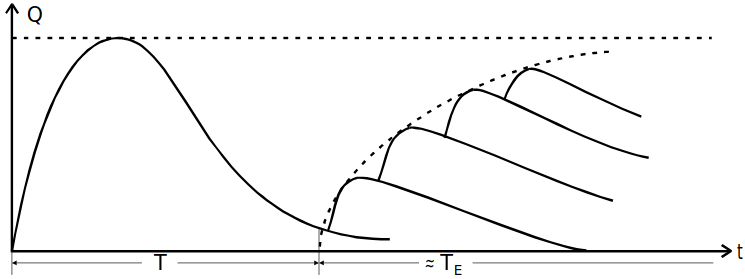
\includegraphics[width = 0.7\linewidth]{totzeit_erholungszeit.png}
            \caption{Die Ladungsimpulse gegen die Zeit aufgetragen, um die Tot- und Erholungszeit darzustellen.}
            \label{fig:totzeit_erholungszeit}
          \end{figure}
          \FloatBarrier

          Kommen die Ionen am Zählrohrmantel / der Kathode an, so wird bei ihrer Neutralisation genug Energie frei, dass sie Elektronen aus der Kathode lösen können. Durch die dadurch erzeugten Sekundärelektronen enstehen mehrere zeitlich versetzte Ladungsimpulse, die Nachentladungen genannt werden. Diese täuschen ein einfallendes Teilchen vor und verfälschen somit die Messung. Um dies zu vermeiden werden Alkoholdämpfe zum Edelgas in den Stahlzylinder gemischt. Die Alkoholmoleküle haben eine geringere Ionisierungsenergie als die Gasatome, weshalb bei Zusammenstößen miteinander die Ersteren ionisiert werden. Die Alkoholmoleküle bewegen sich anstelle der Gasatome zur Kathode wo sie neturalisiert werden. Die dadurch freigesetzte Energie reicht nicht mehr aus um Elektronen aus der Kathode zu entfernen, da die Energie von den Schwingungen der vielatomigen Alkoholmoleküle verbraucht wird. Somit ist das Problem der Nachentladung gelöst.

        \subsubsection{Charakteristik des Zählrohrs}
          Wenn bei konstanter Intensität die Anzahl der registrierten Teilchen $N$ gegen die Spannung $U$ aufgetragen wird kann die Charakteristik eines Geiger-Müller-Zählrohrs bestimmt werden. Der Auslösebereich fängt bei der Spannung $U_{\text{E}}$ an. Danach gibt es einen linearen Teil: das Plateau. Bei einem idealen Zählrohr wäre die Steigung des Plateaus gleich null. In der Realität lassen sich jedoch nicht alle Nachentladungen vermeiden, die mit steigender Spannung zunehmen. Deswegen hat das Plateau eine Steigung. Je geringer die Steigung und je länger das Plateau, desto qualitativ hochwertiger ist das Zählrohr.

          Nach dem Plateau nehmen die Nachentladungen sehr stark zu, was zu einer Dauerentladung führt.

        \subsubsection{Ansprechvermögen des Zählrohrs}
          Darunter wird die Wahrscheinlichkeit verstanden, dass ein einfallendes Teilchen im Zählrohr registriert wird. Aufgrund des hohen Ionisationsvermögens der $\alpha$- und $\beta$-Teilchen werden sie so gut wie zu 100$\%$ detektiert. Anders sieht es bei den $\gamma$-Quanten aus. Da Photonen nicht geladen sind und hochenergetische Photonen nur sehr wenig mit Materie wechselwirken liegt das Ansprechvermögen bei ca. 1$\%$. Deshalb ist es nur sinnvoll das Geiger-Müller-Zählrohr einzusetzenm, wenn die $\gamma$-Strahlung niederenergetisch ist und/oder eine hohe Intensität hat.

        \subsubsection{Totzeitmessung mit der Zwei-Quellen-Methode}
          Die Totzeit ist die Zeit in der nach einem registrierten Ereignis keine weiteren Ereignisse registriert werden können. Die Totzeitkorrektur ist dann anzuwenden, wenn die Zählrate $n$ groß im Vergleich zur Totzeit $T$ ist. Dann gilt für die wahre Zählrate $n^*$ vereinfachend:
          \begin{equation}
            n^* = \frac{n}{1 - t n}
            \label{eqn:totzeit}
          \end{equation}
          Bei der Zwei-Quellen-Methode werden, wie der Name schon sagt, zwei radioaktive Präparate benutzt. Es werden nacheinander erst die Zählrate eines Präparates $n_1$, die Zählrate des Anderen $n_2$ und die Zählrate beider Präparate zusammen $n_{1+2}$ aufgenommen. Dabei sollen die Präparate einen eigenen Platz relativ zum Zählrohr haben der während der Messungen gleich bleibt. Theoretisch sollte ohne Totzeit $n_{1+2} = n_1 + n_2$ gelten. Doch mit der Totzeit gilt, da beide Präparate gemeinsam eine höhere Intensität und deshalb die Totzeit öfter ausgelöst wird:  $n_{1+2} < n_1 + n_2$.

          Mit \autoref{eqn:totzeit} für $n^*_1$, $n^*_2$ und $n^*_{1+2}$ und $n^*_{1+2} = n^*_1 + n^*_2$ gilt nach Umformung $T$ näherungsweise:
          \begin{equation}
            T \approx \frac{n_1  + n_2 - n^*_{1+2}}{2 n_1 n_2}
            \label{eqn:zwei_quellen_methode_totzeit}
          \end{equation}
          
    
    \section{Durchführung}
      Es wird ein Versuchaufbau wie in \autoref{} verwendet. Dabei fließt der Ionisationsstrom über den Anodendraht ab und erzeugt einen Spannungsimpuls, welcher über den Kondensator abgekoppelt wird, wenn nötig vergrößert wird und mit einem Zählgerät registriert wird.
      \begin{figure}[h]
        \centering
        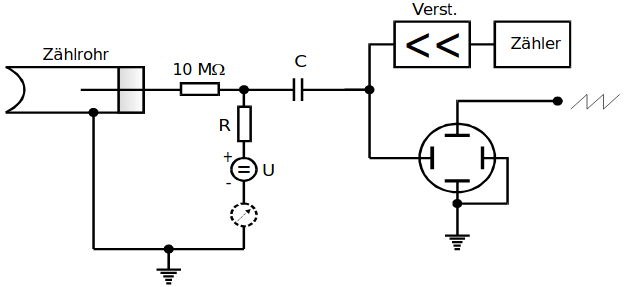
\includegraphics[width = 0.7\linewidth]{Versuchsaufbau.png}
        \caption{Ein schematischer Versuchsaufbau, um die nötigen Messwerte aufzunehmen.}
        \label{fig:totzeit_erholungszeit}
      \end{figure}
      \FloatBarrier

        \subsection{Messung zur Bestimmung der Charakteristik des Zählrohrs}
        Eine $\beta$-Quelle wird vor das Eintrittsfenster des Zählrohrs gestellt und es wird die Anzahl der registrierten Teilchen in Abhängigkeit der Betriebsspannung in 10V Schritten gemessen. Dabei soll die Intensität der Strahlung niedrig sein / die Zählrate sollte nicht größer als 100/s sein, um die Totzeitkorrektur zu vermeiden, da diese nur bei, im Vergleich zur Totzeit, großen Zählraten Sinn macht.

        Da die Plateausteigung sehr gering ist müssen die Messwerte auch sehr genau sein. Es wird eine so lange Interationszeit (in diesem Fall $T = 60$s) genommen, dass der relative statistische Fehler jedes Messwertes unter $1 \%$ liegt. Damit ist die Anzahl der registrierten Teilchen relativ hoch.

      \subsection{Bestimmung der Ladung pro einfallendem Teilchen}
        Während der Aufnahme der Kennlinie wird der Zählstrom / Ionisationsstrom in 50V Schritten gemessen. Die Ablesegenauigkeit am Amperemeter ist $\Updelta I = 0,05 \mu$s.

      \subsection{Messung zur Bestimmung der Totzeit}
        \paragraph{Mit der Zwei-Quellen-Methode:}
          Um die Intensität und damit die Zählrate zu steigern, um eine sinvolle Totzeitkorrektur durchzuführen werden die beiden Quellen nah an das Zählrohr plaziert. Um die Messung möglichst genau zu machen, beträgt die Integrationszeit $T = 120$s.
        \paragraph{Mithilfe des Oszilloskopen:}
          Hierbei werden wie schon vorher erwähnt, die Ladungsimpulse am Oszilloskopen gegen die Zeit aufgetragen, damit nach \autoref{fig:totzeit_erholungszeit} die Totzeit abgelesen werden kann.

    
    \newpage
    \section{Auswertung}
      \subsection{Charakteristik des Zählrohres}
      \begin{figure}[h]
        \centering
        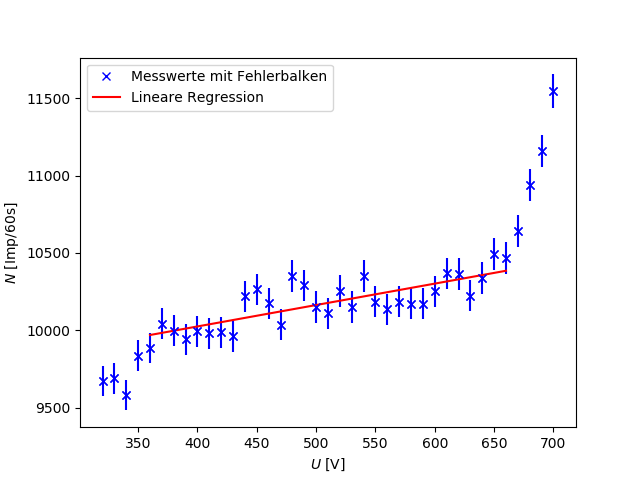
\includegraphics[width = 0.8\linewidth]{Plateau.png}
        \caption{Die Zählrate gegen die Zählrohrspannung aufgetragen.}
        \label{fig:totzeit_erholungszeit}
      \end{figure}
      \FloatBarrier
      
      Da die Zählraten Poisson verteilt sind, gilt für die Messunsicherheiten der Werte der Kennlinie $\Updelta n = \sqrt{n}$. Durch die Messpunkte des Plateaus wird eine Gerade mit der Steigung $m$ und dem y-Achsenabschnitt $b$ durchgeführt: $n(U) = m \cdot U + b$. Die Steigung der Geraden beträgt:
      \begin{equation}
        m = 1,39 \pm 0,04 \frac{1}{\text{V}}
      \end{equation}
      Hiermit wird die Plateausteigung $S$ in $\%$ pro 100V bestimmt. Dazu werden zwei Spannungen mit 100V Differenz im Plateau ausgewählt wie z.B. $U_\text{a} = 400$V und $U_\text{e} = 500$V. Mit diesen Werten wird dann anhand folgender Formel die Steigung berechnet.
      \begin{equation}
        S = \frac{n(U_\text{e}) - n(U_\text{a})}{n(U_\text{e})} \cdot 100 \%
        \label{eqn:steigung_1}
      \end{equation}
      Oder es wird die etwas umgeschriebene Form von \autoref{eqn:steigung_1} benutzt:
      \begin{equation}
          S = 100\text{V} \cdot \frac{m}{n(U_\text{e})} \cdot 100 \% = 1,36 \pm 0,04 \%
      \end{equation}

    \subsection{Bestimmung der Totzeit}
      \subsubsection{Oszilloskop}
        Hierbei wird die Zeit zwischen dem ersten und zweiten Impuls so gut wie möglich abgelesen.
        \begin{figure}[h]
          \centering
          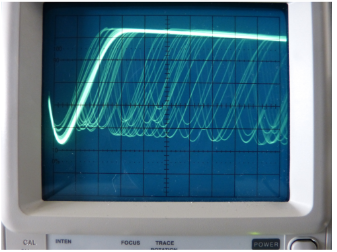
\includegraphics[width = 0.7\linewidth]{Oszilloskop_Geiger_Mueller.png}
          \caption{Eine Momentaufnahme eines Oszilloskopen der Ladung gegen die Zeit aufgetragen. Ein Kästchen sind dabei $100 \mu$s.}
          \label{fig:totzeit_erholungszeit}
        \end{figure}
        \FloatBarrier
        Die abgelesene Totzeit beträgt ca. $T = 100 \mu$s.
      \subsubsection{Zwei-Quellen-Methode}
        Für der erste Präparat, das zweite Präparat und für beide Präparate zusammen wurden die folgenden Zählraten gemessen:
        \begin{align*}
          N_1 &= 96041 \pm 310 \, \text{Imp} \\
          N_2 &= 76518 \pm 277 \, \text{Imp} \\
          N_{1+2} &= 158479 \pm 398 \, \text{Imp}
        \end{align*}
        Zuerst werden die Anzahlen der Ladungsimpulse anhand von $n = N / 60$s in Zählraten umgewandelt:
        \begin{align*}
            n_1 &= 1601 \pm 5 \, \text{Imp/s} \\
            n_2 &= 1275 \pm 5 \, \text{Imp/s} \\
            n_{1+2} &= 2641 \pm 7 \, \text{Imp/s}
          \end{align*}
        Mit \autoref{eqn:zwei_quellen_methode_totzeit} wird dann die Totzeit
        \begin{equation*}
          T \approx (115 \pm 5) \, \mu\text{s}
        \end{equation*}
        berechnet.

    \subsection{Bestimmung der Ladung pro einfallendem Teilchen}
      Hier wird anhand folgender Formel
      \begin{equation*}
          Z = \frac{I}{e \cdot n}
      \end{equation*}
      wo $I$ der Ionisationsstrom, $e$ die Elementarladung, $n$ die Zählrate und $Z$ die pro einfallendem Teilchen freigesetzte Ladung ist.
      \begin{table}[h]
        \centering
        \caption{Hier sind die Messwerte der Spannung $U$ , der Zählrate $n$, der pro einfallendem Teilchen freigesetzer Ladung $Z$ und ihre Messunsicherheiten dargestellt.}
        \label{tab:Ladungen}
        \begin{tabular}{c c c}
          \toprule
          {$I$ [nA]} & {$n$ [1/s]} & {$Z$ [$e \cdot 10^{10}$]} \\
          \midrule
          $300 \pm 50$ & $164 \pm 2$ & $1,14 \pm 0,19$\\
          $400 \pm 50$ & $167 \pm 2$ & $1,50 \pm 0,19$\\
          $700 \pm 50$ & $171 \pm 2$ & $2,55 \pm 0,18$\\
          $800 \pm 50$ & $169 \pm 2$ & $2,95 \pm 0,19$\\
          $1000 \pm 50$ & $170 \pm 2$ & $3,68 \pm 0,19$\\
          $1300 \pm 50$ & $171 \pm 2$ & $4,75 \pm 0,19$\\
          $1400 \pm 50$ & $175 \pm 2$ & $5,00 \pm 0,18$\\
          $1800 \pm 50$ & $192 \pm 2$ & $5,84 \pm 0,17$\\
          \bottomrule
        \end{tabular}
      \end{table}
      \FloatBarrier

      Jetzt wird die pro einfallendem Teilchen freigesetzer Ladung gegen die Spannung aufgetragen
      \begin{figure}[h]
        \centering
        \includegraphics[width = 0.7\linewidth]{Ladungen.png}
        \caption{Die pro einfallendem Teilchen freigesetzer Ladung gegen die Spannung aufgetragen.}
        \label{fig:ladungen}
      \end{figure}
      \FloatBarrier
    
      und es ist erkennbar, dass es einen linearen Zusammenhang zwischen den beiden Größen gibt.

    \newpage
    \section{Diskussion}
      Bei der Analyse des Plateaus wurde eine Plateausteigung von $S = = 1,36 \pm 0,04 \%$ bestimmt. Außerdem ist es am Graphen abzulesen, das der Plateaubereich von ca. 350V bis 650V geht. Dadrüber liegt der zuvermeidende Entladungsbereich und dadrunter der Proportionalbereich.

      Die mit den beiden Methoden bestimmten Totzeiten liegen in der erwarteten Größenordnung von $100 \mu$s.

      Die pro einfallendem Teilchen freigesetze Ladung ist, wie es an \autoref{fig:ladungen} zu erkennen ist proportional zur Spannung.

      Alles in allem wurden die theoretisch erwateten Eigenschaften des Geiger-Müller-Zählrohr durch die Messungen bestätigt.

          
    \newpage
    \section{Daten}
    \begin{table}[h]
      \centering
      \caption{Das sind die Messwerte der Zählrate bei einer Integrationszeit von 60s, ihrer Unsicherheit und der Spannung.}
      \label{tab:Kennwerte}
      \begin{tabular}{c l c l}
        \toprule
        U [V] & n [Imp/60s] & U [V] & n [Imp/60s] \\
        \midrule
        320 &	$9672   \pm 99 $ & 520 & $10255  \pm 102$ \\
        330 &	$9689   \pm 99 $ & 530 & $10151  \pm 101$ \\
        340 &	$9580   \pm 98 $ & 540 & $10351  \pm 102$ \\
        350 &	$9837   \pm 100$ & 550 & $10184  \pm 101$ \\
        360 &	$9886   \pm 100$ & 560 & $10137  \pm 101$ \\
        370 &	$10041  \pm 101$ & 570 & $10186  \pm 101$ \\
        380 &	$9996   \pm 100$ & 580 & $10171  \pm 101$ \\
        390 &	$9943   \pm 100$ & 590 & $10171  \pm 101$ \\
        400 &	$9995   \pm 100$ & 600 & $10253  \pm 102$ \\
        410 &	$9980   \pm 100$ & 610 & $10368  \pm 102$ \\
        420 &	$9986   \pm 100$ & 620 & $10365  \pm 102$ \\
        430 &	$9960   \pm 100$ & 630 & $10224  \pm 102$ \\
        440 &	$10219  \pm 102$ & 640 & $10338  \pm 102$ \\
        450 &	$10264  \pm 102$ & 650 & $10493  \pm 103$ \\
        460 &	$10174  \pm 101$ & 660 & $10467  \pm 103$ \\
        470 &	$10035  \pm 101$ & 670 & $10640  \pm 104$ \\
        480 &	$10350  \pm 102$ & 680 & $10939  \pm 105$ \\
        490 &	$10290  \pm 102$ & 690 & $11159  \pm 106$ \\
        500 &	$10151  \pm 101$ & 700 & $11547  \pm 108$ \\
        510 &	$10110  \pm 101$ \\
        \bottomrule
      \end{tabular}
    \end{table}

        \newpage
        \section{Literaturverzeichnis}
        [1] \textit{Versuchsanleitung V703 - Das Geiger-Müller-Zählrohr.} TU Dortmund, 2020 \newline
        [2] Physical Measurement Laboratory: \textit{X-Ray Transition Energies Database} 10. Mai 2020
        \url{https://physics.nist.gov/PhysRefData/XrayTrans/Html/search.html} \newline
        [3] The NIST Reference on Constants, Units and Uncertainty: \textit{Fundamental Physical Constants} 10. Mai 2020
        \url{https://physics.nist.gov/cgi-bin/cuu/Value?ecomwl|search_for=atomnuc!}

\end{document}

